The marine ecosystem model used in this study is the Apex Predators Ecosystem Model (Apecosm, \citealt{mauryModelingEnvironmentalEffects2007, mauryOverviewAPECOSMSpatialized2010}), which simulates the transfer of energy in marine ecosystems in a 5 dimensional space (space, time, community and size). The biological processes include size-based opportunistic trophic interactions, competition for food, allocation of energy between growth and reproduction, somatic and maturity maintenance, predatory and starvation mortality (see \citealt{mauryModelingEnvironmentalEffects2007} for a detailed description of the model). The physiological bases of the model are derived from the Dynamic Energy Budget theory (DEB, \citealt{kooijmanDynamicEnergyMass2000}). All the physiological rates are temperature-dependent. In addition to biological processes, energy density is also subjected to both passive (via ocean currents) and active (foraging behaviour) advection/diffusion, following \cite{faugerasAdvectiondiffusionreactionSizestructuredFish2005}.

Changes of fish biomass induced by growth is given by:

\begin{equation}
\partial_t \varepsilon = - \partial_w(\gamma \varepsilon) + \frac{\gamma}{w}\varepsilon
\label{eq:growth}
\end{equation}

where $\varepsilon$  is the fish biomass density, $w$ the weight and $\gamma$ is the growth rate. Changes driven by predation mortality are given by:

\begin{equation}
\partial_t \varepsilon = - M \varepsilon
\label{eq:pred}
\end{equation}

where $M$ is the predation mortality rate, computed using equation 12 of \cite{mauryIndividualsPopulationsCommunities2013}. 

Finally, changes in fish biomass induced by fish movements are given by:

\begin{equation}
\partial_t \varepsilon = -\overrightarrow{\nabla}.(\overrightarrow{V} \varepsilon) + \overrightarrow{\nabla} . (D \overrightarrow{\nabla} \varepsilon)
\label{eq:move}
\end{equation}

with the first term being the contribution of advection and the second term being the contribution of diffusion, $V$ the velocity and $D$ the diffusivity coefficient.

In order to ensure that the size-spectrum is fully unfolded, the model has been integrated three times. First, the model has been initialized from rest and integrated from 1958 to 2018, using the outputs of the NEMO-PISCES simulation. Then, the end of this first spin-up phase has been used to run another cycle, which was in turn used to run the simulation presented in the following.

In order to assess the mechanisms of fish biomass response to ENSO variability, biomass changes induced by growth, predation, advection and diffusion are stored for the entire simulation. Therefore, the biomass for a given size class, at a given location and for a specific time can be reconstructed by using the following equation:

\begin{equation}
\varepsilon(T) = \varepsilon(T=0) + \int_{t=0}^{T} \left[ 
T_{pred}(t) +
T_{growth}(t) + 
T_{adv}(t) + 
T_{diff}(t) 
\right] dt 
\label{eq:rec_oope}
\end{equation}

with $\varepsilon(x,y,s,T=0)$ the fish biomass at the beginning of the simulation and $T_{pred}$, $T_{growth}$, $T_{adv}$ and $T_{diff}$ the respective biomass increments due to predation, growth, advection and diffusion, given by equations \ref{eq:pred}, \ref{eq:growth} and \ref{eq:move}, respectively.

In the present work, three generic communities are simulated: one epipelagic community, one migrant community and one mesopelagic community. The epilagic community remains close to the surface its vertical distribution is influenced by temperature and oxygen, while light only influences their functional response. The migrants are only influenced by light, which modifies their vertical habitat and their functional response: during daytime, they remain at depth, while moving at the surface at night for feeding. Mesopolagics, on the other hand, remain at depth during both night and day, their vertical distribution being only impacted by the light. 
%Epilagic feed on other epilagic fish only during night daytime. Migrants feed on other migrants and epipelagics, only during night-time. While mesopelagics feed on migrant and mesopelagic during daytime, and only on other mesopelagic during night-time.

Since the epipelagic are close to the surface (around $50m$), they are likely to be more impacted by ENSO variability, as suggested by \cite{lemezoNaturalVariabilityMarine2016}. Therefore, in the following, we will mainly focus on this specific community. 

Before analysing the mechanisms of fish biomass response to El Nino variability, simulated biomass integrated from 30cm to 70cm is compared with the observation-based estimates presented in Section \ref{sec:fish}. Figure \ref{fig:apecosm_validation}a shows the Hovmoller diagram of the observed catches and fish biomass (log-scale) integrated between 10N and 10S for the 2008-2018 period. Although observed and model results cannot be directly compared, some features are well captured by the model. For instance, the easternmost $4.00$ simulated contour seems to closely follow the eastward extensions of catches that occur in 2010, 2012 and 2016. Figure \ref{fig:apecosm_validation}b shows, for a longer period (1985-2018), the longitudinal position of the catch and biomass barycenters. The observed barycenter shows an eastward trend, liley due to the increased power of fishing fleets, which allow them to navigate over greater distances from their fishing ports, mostly located in the western Pacific (\warn{ref}). This emphasizes the fact that the data used in this validation are catch data, which are not only dependent on fish biomass but also depend on fishing effort, and as such must be used with caution for the comparison with simulated fish biomass. Figures \ref{fig:apecosm_validation}c and \ref{fig:apecosm_validation}d show the difference between catch and simulated biomass composites for El Nino (OND2009-JFM2010, OND2014-JFM2015, OND-2015-JFM2016) and La Nina conditions (OND2007-JFM2008, OND2008-JFM2009, OND2010-JFM2011, OND2011-JFM2012). Observed catches increase in the central and eastern Pacific and decrease in the Western Pacific when switching from La Nina to El Nino conditions, which is consistent with an eastward displacement of the fish biomass. Simulated composite also shows an increase in the central Pacific and a decrease in the west, although the pattern seems westward shifted compared with the catch composite. 

\begin{figure}
	\centering
	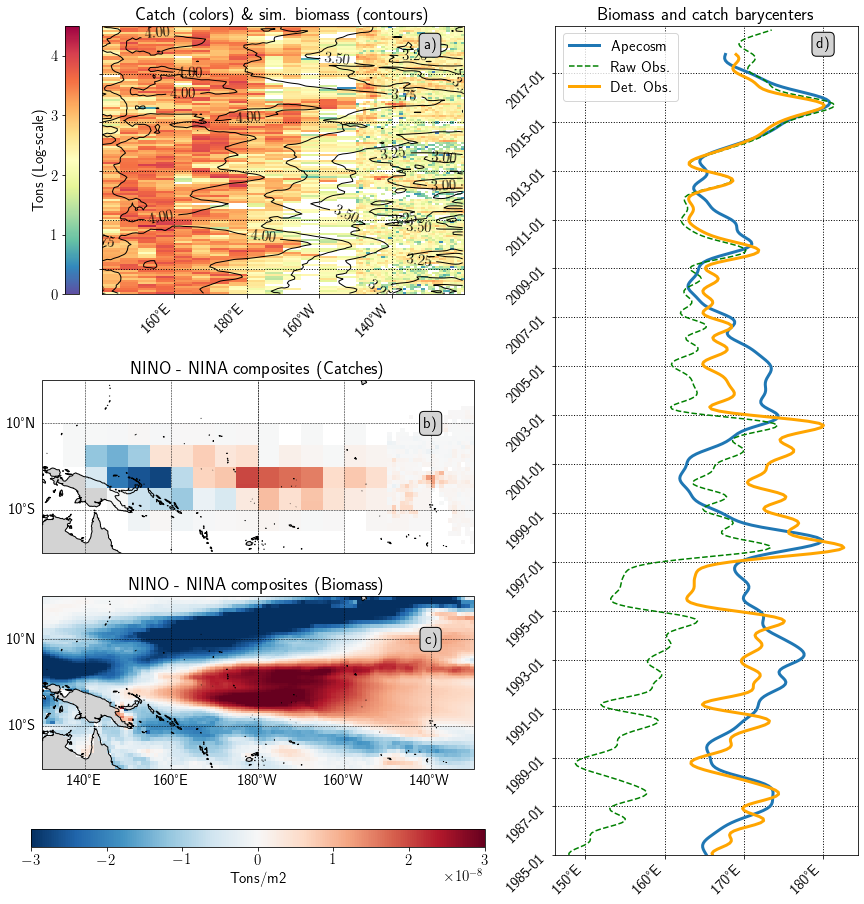
\includegraphics[scale=0.5]{figs/plot_validation_apecosm.png}
	\caption{Hovmoller diagram of observed catches (colors) and simulated fish biomass (contours) integrated between 10N and 10S (a, log-scale) and associated barycenters (b). Catch (c) and simulated fish-biomass (d) difference between El Nino and La Nina composites.}
	\label{fig:apecosm_validation}
\end{figure}

In the following, the results for three size classes, 3cm, representing small fishes, 20cm, representing intermediate sizes, and 90 cm, representing large individuals, will be detailed. The latter are representative of the sizes of tuna target species within the region (\warn{REF}). \\
